\documentclass[20pt]{article}
\usepackage{amssymb}
\usepackage{amsmath}
\usepackage{setspace}
\usepackage{graphicx}
\begin{document}
\title{Finding Area}
\maketitle
\author{CVS KUSAL REDDY EE17BTECH11012}\\{P SUNIL VARMA EE17BTECH11026}



\section{Question}
 If an equlateral triangle, having centroid at the
origin, has a side along the line
(1 1)x = 2,then find the area of this triangle. 
\section{solution}
Given line equation of one side is \\
\[ 
\begin{bmatrix}
 1 & 1 \\
\end{bmatrix}X = 2
\]
 and centroid is at origin O(0,0).\\
 Since it is an equilateral triangle,
 the perpendicular distance between centroid and any side = $\frac{a}{2\sqrt{3}}$     
\begin{flushright}
 where a is side length of triangle
\end{flushright} 
The perpendicular distance between point ($x_{1}$,$y_{1}$)  and straight line ax+by+c=0 
is given by $\frac{ax_{1} +by_{1}+c}{\sqrt{a^{2}+b^{2}}}$ \\ 
let d be the perpendicular distance \\
\begin{center}
d = $\frac{|1(0)+1(0)-2|}{\sqrt{1^{2}+1^{2}}}$\\
\singlespacing
 d = $\frac{2}{\sqrt{2}}$\\
\singlespacing
  d = $\sqrt{2}$    \\
\singlespacing
 From above we know that
\singlespacing
d=$\dfrac{a}{2\sqrt{3}}$\\
\singlespacing 
   a=2d$\sqrt{3}$\\
\singlespacing
The area of equilateral is $\dfrac{\sqrt{3}a^{2}}{4}$ \\
\singlespacing  
  Area  = 3$\sqrt{3}d^{2}$  \\
\singlespacing 
  Area = 3$\sqrt{3}(\sqrt{2})^{2}$\\
\singlespacing  
  Area = 6$\sqrt{3}$\\
\singlespacing
The figure of perpendicular from centroid to side of triangle
 
\end{center}
\begin{figure}[h]
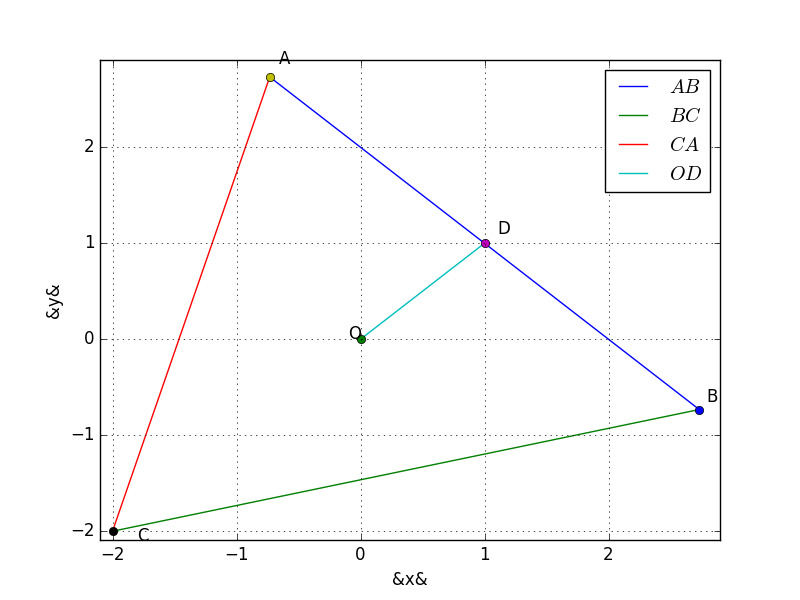
\includegraphics[scale=0.75]{figure_1}
\caption{perpendicular from centroid}
\end{figure}
  \end{document}